\chapter{Rulial Space \& Rulial Distance}
\label{chapter-5-rulial-space-rulial-distance}

\section{The Shape of Possibility}
\label{the-shape-of-possibility}

The moment you start thinking about computation not as code, not as functions, not as instructions, but as \textbf{rewrite}, everything you thought was ``time'' or ``logic'' or ``behavior'' begins to collapse into something more elemental:

\textbf{Possibility.}

Up to now, we have been walking a single path—a worldline. This is the path the scheduler chose, the specific sequence the rules allowed, and the history that actually happened. It is the linear narrative we see in our log files and standard debuggers.

But this chapter is about something far more interesting: \textbf{All the other paths you could have taken.}

We are not discussing infinite branching sci-fi scenarios, nor are we invoking metaphysical multiverses or the totality of Wolfram's Ruliad. We are strictly concerned with the \textbf{local neighborhood} around the computation you are inhabiting right now. This neighborhood consists of the legal next rewrites, the immediate futures, and the adjacent alternative worlds. It represents the doors in the room you are standing in, regardless of whether you choose to open them.

Crucially, this neighborhood has structure. It has a shape. It possesses direction, boundaries, and curvature. And—most importantly—it has a \textbf{finite, computable geometry}.

This is the geometry of thought. This is the shape of possibility.

Welcome to \textbf{Rulial Space}.

\begin{center}
\rule{0.5\linewidth}{0.5pt}
\end{center}

\section{From Rewrites to Possibility}
\label{from-rewrites-to-possibility}

At any specific moment in a Recursive Meta-Graph (RMG) universe, the system is vibrant with potential. A set of Double-Pushout (DPO) rules is waiting to fire.

The behavior of these rules is rarely uniform. Some rules match the current graph topology immediately. Others fail to match. Some conflict with one another, fighting for the same resources, while others overlap peacefully. There are rules that are impossible in the current tick but will become inevitable in the next, and rules that rewrite deeply nested structures inside an edge or a node.

When you take all these potential interactions together, they do not form a chaotic cloud. They form a \textbf{finite set of legal next moves}.

This set is the \textbf{local slice} of Rulial Space. It is the subgraph of all reachable RMG states exactly one tick away from the current worldline, bounded strictly by your specific rule system. We call this the \textbf{Kairos plane}—the field of immediate legal options.

You feel the presence of this plane every time you write code, debug a complex system, or attempt to optimize a pipeline. You are intuitively navigating possibility, sensing which moves are legal and which are blocked. This chapter provides the formal language to make that intuition explicit.

\begin{center}
\rule{0.5\linewidth}{0.5pt}
\end{center}

\section{Chronos, Kairos, Aios: The Three Axes of Computation}
\label{chronos-kairos-aios-the-three-axes-of-computation}

Modern software engineering suffers from a temporal myopia; it generally possesses only one notion of time, which is the step that just happened. However, thinking in terms of graph rewrites reveals a much richer, three-dimensional picture of computational existence.

\subsection{Chronos — The Worldline You Actually Took}
This is the axis of history. It represents the deterministic, tick-by-tick execution that brought the system to its current state. It is the linear path behind you, the committed decisions, and the immutable logs.

\subsection{Kairos — The Time Cube}
This is the axis of opportunity. Kairos represents the shape of legal next steps from the present moment. It is the local cone of possibility, the width of the choice you have right now before the scheduler collapses it into history.

\subsection{Aios — The Structural Arena}
This is the axis of permanence. Aios is the structural hull carved out by the rule algebra itself. It is not the set of states you will ever reach, but the set of states that are even legal under your rewrite physics. Aios defines the universe's computable boundary conditions.

\begin{figure}[h]
\centering
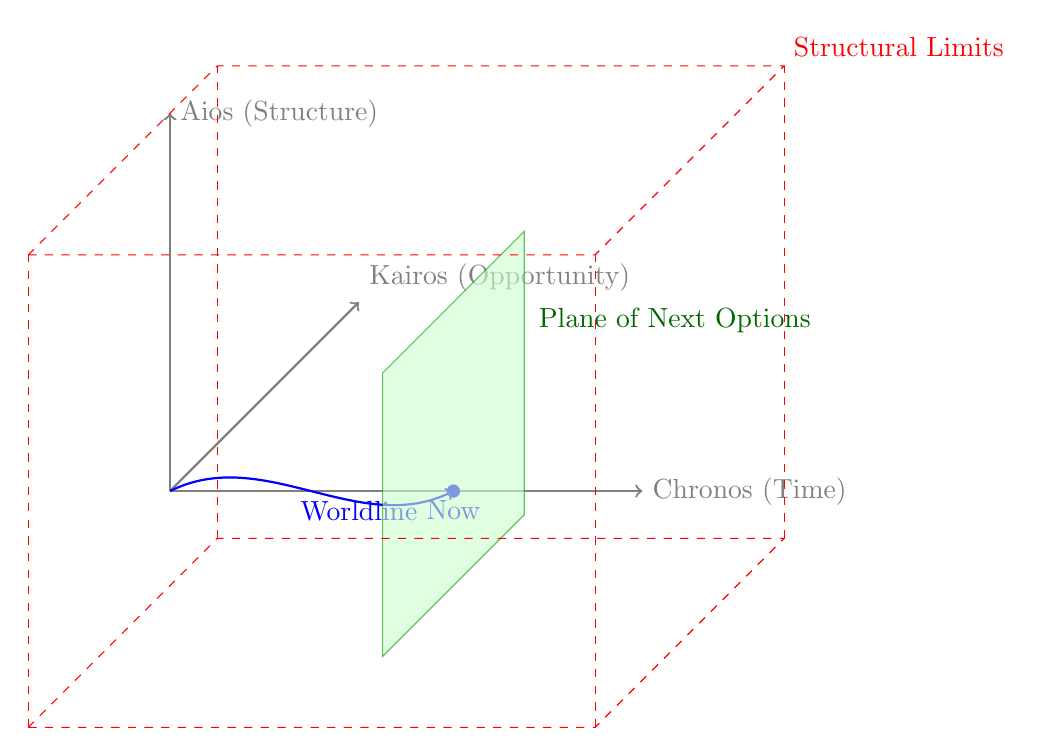
\begin{tikzpicture}[scale=1.2, x={(1cm,0cm)}, y={(0.5cm,0.5cm)}, z={(0cm,1cm)}]
    % Draw Axes
    \draw[->, thick, gray] (0,0,0) -- (5,0,0) node[anchor=west]{Chronos (Time)};
    \draw[->, thick, gray] (0,0,0) -- (0,4,0) node[anchor=south west]{Kairos (Opportunity)};
    \draw[->, thick, gray] (0,0,0) -- (0,0,4) node[anchor=west]{Aios (Structure)};

    % Draw Chronos Path
    \draw[blue, thick, ->] (0,0,0) .. controls (1,0,0.5) and (2,0,-0.5) .. (3,0,0);
    \node[blue, below] at (2,0,0) {Worldline};
    \fill[blue] (3,0,0) circle (2pt) node[anchor=north] {Now};

    % Draw Kairos Plane at "Now" (Visualized as a vertical slice)
    \filldraw[fill=green!20, opacity=0.6, draw=green!60!black] 
        (3,-1.5,-1) -- (3,1.5,-1) -- (3,1.5,2) -- (3,-1.5,2) -- cycle;
    \node[green!40!black, anchor=west] at (3, 1.6, 1) {Plane of Next Options};

    % Draw Aios Boundary (Wireframe Hull)
    \draw[red, dashed] (-0.5,-2,-1.5) -- (5.5,-2,-1.5) -- (5.5,2,-1.5) -- (-0.5,2,-1.5) -- cycle; % Bottom
    \draw[red, dashed] (-0.5,-2,3.5) -- (5.5,-2,3.5) -- (5.5,2,3.5) -- (-0.5,2,3.5) -- cycle; % Top
    \draw[red, dashed] (-0.5,-2,-1.5) -- (-0.5,-2,3.5);
    \draw[red, dashed] (5.5,-2,-1.5) -- (5.5,-2,3.5);
    \draw[red, dashed] (5.5,2,-1.5) -- (5.5,2,3.5);
    \draw[red, dashed] (-0.5,2,-1.5) -- (-0.5,2,3.5);
    
    \node[red, anchor=south west] at (5.5, 2, 3.5) {Structural Limits};

\end{tikzpicture}
\caption{The Three Axes of Computation. Chronos tracks the history, Kairos defines the immediate future possibilities, and Aios bounds the structural laws of the universe.}
\end{figure}

This three-way model allows us to express the totality of a program's life. We can differentiate between what actually happened (Chronos), what could happen next (Kairos), and what is even possible in the first place (Aios). To navigate computation consciously, you must be aware of all three dimensions.

\begin{center}
\rule{0.5\linewidth}{0.5pt}
\end{center}

\section{The Time Cube: A Local Lens on Rulial Space}
\label{the-time-cube-a-local-lens-on-rulial-space}

You can visualize the immediate future not just as a list of options, but geometrically as a \textbf{Time Cube}—or more accurately, a \textbf{cone of possible futures}.

When your worldline (Chronos) hits a specific moment, the single point of ``now'' expands. From that point, a fan of legal DPO rewrites opens outward. This cone is defined by specific properties: it is \textbf{finite}, because only legal rewrites count; it is \textbf{local}, because it depends entirely on the current state; and it is \textbf{computable}, meaning we can strictly enumerate every lawful match.

Before we proceed, we must clarify who is actually looking at this cone. This distinction will save you significant headaches in later chapters.

\vspace{0.5cm}
\begin{center}
\fbox{
    \begin{minipage}{0.9\textwidth}
    \textbf{Note: Observer vs. Scheduler vs. System}
    
    To understand Rulial Space, you must separate the machinery from the measurement:
    \begin{itemize}
        \item \textbf{The System} (the rewrite substrate) does not ``see'' alternate universes. It simply \emph{is}.
        \item \textbf{The Scheduler} is the logic that walks the path. It samples the rule bundle and commits to exactly one admissible rewrite at a time. It produces the Worldline.
        \item \textbf{The Observer} is the external interpretive frame—you, the developer, the debugger, or the formal agent. The Observer is the only entity that sees the whole maze, compares worldlines, and measures the geometry.
    \end{itemize}
    The System executes \emph{one} worldline. Only the Observer perceives Rulial curvature and distance. The Scheduler merely walks.
    \end{minipage}
}
\end{center}
\vspace{0.5cm}

The Time Cube is the lens through which the \textbf{Observer} sees where the Scheduler \textit{could} go next. It reveals that you cannot go everywhere; you can only reach the nearby computational futures allowed by the geometry of the graph.

\begin{center}
\rule{0.5\linewidth}{0.5pt}
\end{center}

\section{Rulial Distance: The Metric on Possibility}
\label{rulial-distance-the-metric-on-possibility}

If Rulial Space is the arena of all reachable states, how do we measure the space between them? We need a metric. We need \textbf{Rulial Distance}.

The definition is beautifully simple:

\begin{quote}
\textbf{The Rulial Distance between two states is the minimal number of legal rewrites needed to transform one into the other.}
\end{quote}

To make this concrete, let us abandon abstract graphs and use a tangible example we will return to throughout this book: the **Life-Block**. Imagine a tiny, 3x3 binary grid universe with two simple rules:

\begin{itemize}
    \item \textbf{Rule A (Spawn):} An empty cell fills (0 $\to$ 1) if it has exactly 2 horizontal neighbors.
    \item \textbf{Rule B (Decay):} An active cell empties (1 $\to$ 0) if it has 0 neighbors.
\end{itemize}

For clarity, ``horizontal neighbors'' refers strictly to the left and right adjacent cells. Rule B considers all 4 orthogonal neighbors (up, down, left, right). For edge cells, neighbors outside the 3×3 grid are treated as nonexistent and therefore do not count as active neighbors. This intentionally asymmetric rule set makes the geometry easier to visualize while still producing meaningful curvature.

Consider a transition between two states in this universe. If we start with a horizontal line of three blocks, applying Rule B to the center block is illegal (it has neighbors). However, applying Rule A to the cells above and below the center is legal.

\begin{figure}[h]
\centering
\begin{tikzpicture}[
    gridnode/.style={rectangle, draw=black!50, fill=white, minimum size=0.5cm, outer sep=0pt},
    active/.style={fill=black!80},
    arrow/.style={->, thick, shorten >=2pt, shorten <=2pt}
]

    % Matrix 1: Start State
    \matrix[matrix of nodes, nodes={gridnode}, row sep=-\pgflinewidth, column sep=-\pgflinewidth] (m1) {
        0 & 0 & 0 \\
        |[active]| 1 & |[active]| 1 & |[active]| 1 \\
        0 & 0 & 0 \\
    };
    \node[above=0.1cm of m1] {State $S_0$ (Line)};

    % Matrix 2: Intermediate State
    \matrix[matrix of nodes, nodes={gridnode}, row sep=-\pgflinewidth, column sep=-\pgflinewidth, right=2.5cm of m1] (m2) {
        0 & |[active]| 1 & 0 \\
        |[active]| 1 & |[active]| 1 & |[active]| 1 \\
        0 & 0 & 0 \\
    };
    \node[above=0.1cm of m2] {State $S_1$};

    % Matrix 3: Goal State
    \matrix[matrix of nodes, nodes={gridnode}, row sep=-\pgflinewidth, column sep=-\pgflinewidth, right=2.5cm of m2] (m3) {
        0 & |[active]| 1 & 0 \\
        |[active]| 1 & |[active]| 1 & |[active]| 1 \\
        0 & |[active]| 1 & 0 \\
    };
    \node[above=0.1cm of m3] {State $S_2$ (Cross)};

    % Transitions
    \draw[arrow] (m1) -- node[midway, above] {Rule A (Top)} (m2);
    \draw[arrow] (m2) -- node[midway, above] {Rule A (Bottom)} (m3);
    
    % Distance Label
    \draw[decorate, decoration={brace, amplitude=10pt, mirror}, yshift=-5pt] 
    ($(m1.south west)$) -- ($(m3.south east)$) node [midway, below=15pt] {\textbf{Rulial Distance = 2}};

\end{tikzpicture}
\caption{Rulial Distance in the Life-Block Universe. To transform the line ($S_0$) into the cross ($S_2$) requires two distinct, legal rewrite steps. $S_0$ and $S_2$ are neighbors, but they are not adjacent.}
\end{figure}

If you want to move from the Line ($S_0$) to the Cross ($S_2$), the Rulial Distance is exactly 2. You cannot do it in one step. If you want to move from $S_0$ to an empty grid, you might have to traverse a long chain of Decay rules. And importantly, if you want to move from $S_0$ to a checkerboard pattern, the distance might be \textbf{infinite}—if no sequence of rules exists to produce that pattern, it is structurally forbidden.

Rulial Distance allows us to quantify software behavior structurally. A bug is ``far'' from the correct behavior if it requires a long sequence of improbable state mutations to occur. An optimization is a ``near'' rewrite if it preserves the fundamental shape of the data.

\begin{center}
\rule{0.5\linewidth}{0.5pt}
\end{center}

\section{Curvature: When the Cone Bends Against You}
\label{curvature-when-the-cone-bends-against-you}

Curvature in Rulial Space is not physical curvature in the Einsteinian sense. In the context of the COMPUTER model, curvature is best understood through an analogy to chemistry: \textbf{Activation Energy}.

In chemical kinetics, certain transformations proceed readily (downhill), while others require enormous activation energy to occur. Rulial curvature plays an analogous role in computation:

\begin{itemize}
    \item \textbf{Low Curvature:} State transitions occur through short sequences of permissible rewrites. These are ``downhill'' reactions. The code feels fluid, and refactoring is easy.
    \item \textbf{High Curvature:} Transitions require long, delicate chains of specific rule applications. You must pass through unstable intermediate forms to reach the desired state. This is an ``uphill'' battle against the rule algebra.
    \item \textbf{Infinite Curvature:} The transition is forbidden by the rules. It is like trying to spontaneously turn water into gold.
\end{itemize}

High curvature corresponds to high algorithmic effort: the number of rule applications required to escape a configuration is proportional to the curvature around it.

\begin{figure}[h]
\centering
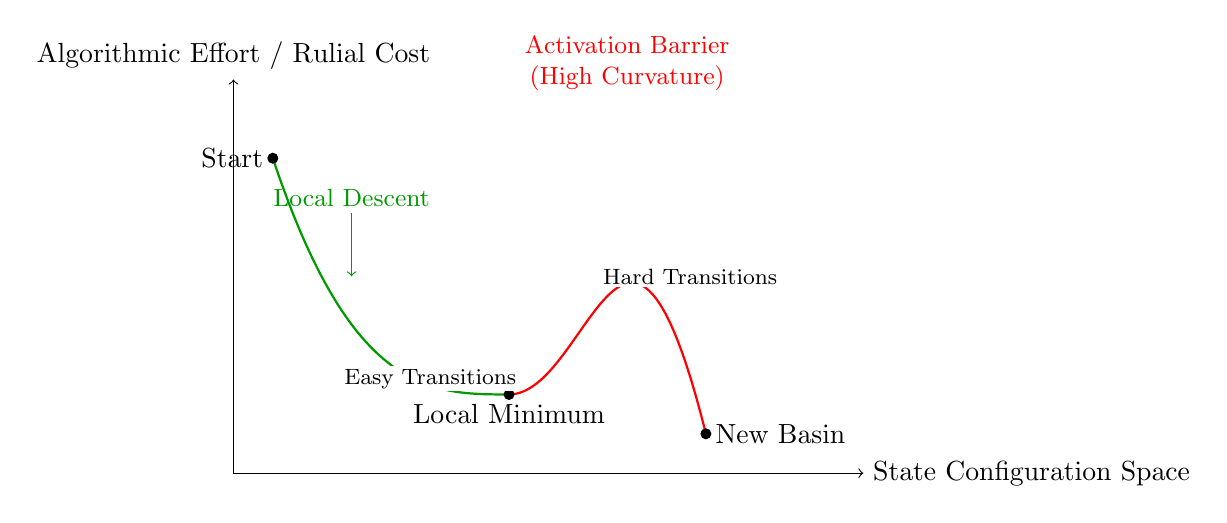
\begin{tikzpicture}
    % Axes
    \draw[->] (0,0) -- (8,0) node[right] {State Configuration Space};
    \draw[->] (0,0) -- (0,5) node[above] {Algorithmic Effort / Rulial Cost};

    % Low Curvature Path (Basin 1)
    \draw[thick, green!60!black] (0.5, 4) .. controls (1.5, 1) and (2.5, 1) .. (3.5, 1);
    \node[green!60!black, font=\small] at (1.5, 3.5) {Local Descent};
    \draw[->, green!60!black] (1.5, 3.3) -- (1.5, 2.5);

    % Activation Barrier
    \draw[thick, red] (3.5, 1) .. controls (4.5, 1) and (5, 4.5) .. (6, 0.5);
    \node[red, font=\small, align=center] at (5, 5.2) {Activation Barrier\\(High Curvature)};
    
    % States
    \fill (0.5, 4) circle (2pt) node[left] {Start};
    \fill (3.5, 1) circle (2pt) node[below] {Local Minimum};
    \fill (6, 0.5) circle (2pt) node[right] {New Basin};
    
    % Path Labels
    \node[font=\footnotesize, fill=white, inner sep=1pt] at (2.5, 1.2) {Easy Transitions};
    \node[font=\footnotesize, fill=white, inner sep=1pt] at (5.8, 2.5) {Hard Transitions};

\end{tikzpicture}
\caption{Curvature as Activation Energy. Escaping a local minimum requires traversing high-curvature states (the activation barrier). The height of the barrier represents the algorithmic effort required to unlock the new basin of states.}
\end{figure}

Consider our Life-Block example again. Moving from $S_0$ to $S_1$ (adding one block) is low curvature—it happens immediately if Rule A fires. But imagine a state where Rule A is blocked by a surrounding wall of zeros. To clear that wall, you might need to trigger a Decay rule elsewhere, which triggers another Spawn, which finally clears the space. That is high curvature.

\begin{center}
\rule{0.5\linewidth}{0.5pt}
\end{center}

\section{Storage IS Computation}
\label{storage-is-computation}

We must ground these geometric concepts in a fundamental realization about the nature of the machine.

An RMG stores state. A DPO rewrite transforms state. Therefore, it follows that \textbf{RMG equals storage}, and \textbf{DPO equals computation}. But when you look closer, the distinction vanishes.

\textbf{Storage is simply frozen computation. Computation is simply storage in motion.}

There is no longer a conceptual split between code and data. The Life-Block grid *is* data, but it is also the *program* that generates the next grid.

Rulial Distance is therefore a metric on computation-as-storage. It does not measure ``how different two states look''; it measures the computational work required to turn one frozen computation into another. In other words, it is the metric tensor of the machine's geometry. This is the key that eventually collapses the concepts of ``runtime'' and ``compiler'' into a singular entity, a concept we will explore fully in Part V.

\vspace{1em}
\begin{center}
\fbox{
    \begin{minipage}{0.65\textwidth}
    \centering
    \textit{The geometry of Rulial Space is not a metaphor; it is the operating geometry of computation itself.}
    \end{minipage}
}
\end{center}

\vspace{1.5em}

\begin{center}
\rule{0.4\linewidth}{0.5pt} \raisebox{-2.5pt}{$\boldsymbol{\Omega}$} \rule{0.4\linewidth}{0.5pt}
\end{center}

\section*{For the Nerds™: The Formal Geometry of Rulial Space}
\addcontentsline{toc}{section}{For the Nerds™: The Formal Geometry of Rulial Space}

\begin{center}
\begin{minipage}{0.92\linewidth}
This section collects the formal definitions underlying Rulial Space, Rulial Distance, curvature, worldlines, and the categorical structure of DPO rewriting. None of this is required to follow the main thread of the book, but it provides the mathematical backbone for later chapters on geodesics, confluence, and computational physics.\footnote{There is a deeper conjectural picture in which Rulial Space admits a coarse-grained manifold structure, with an emergent notion of curvature compatible with the metric defined below. We tentatively refer to this as the \emph{Rulial Manifold Conjecture}.}
\end{minipage}
\end{center}

\vspace{1em}

\subsection*{1. State Space and Rewrite Dynamics}

\begin{definition}[State Space]
Let $\mathcal{R}$ be a fixed DPO rule algebra, and let
\[
\mathcal{S} = \{\, s \mid s \text{ is an RMG state legal under } \mathcal{R} \,\}.
\]
We call $\mathcal{S}$ the \emph{Rulial State Space} determined by $\mathcal{R}$. This is the universe carved out by Aios.
\end{definition}

\begin{definition}[One-Step Rewrite / Local Transition]
For $s, t \in \mathcal{S}$ and $r \in \mathcal{R}$, we write
\[
s \xrightarrow{r} t
\]
if $r$ admits a DPO match on $s$ whose pushout complement yields $t$. When the specific rule is irrelevant, we simply write $s \to t$.
\end{definition}

\begin{definition}[Kairos Slice / Local Neighborhood]
For a state $s \in \mathcal{S}$, the \emph{local slice} (or \emph{Time Cube}) is
\[
N(s) = \{\, t \in \mathcal{S} \mid s \to t \,\}.
\]
This is the set of all legal one-step futures the Scheduler could collapse into from $s$.
\end{definition}

\begin{figure}[h]
\centering
\begin{tikzpicture}[
    state/.style={circle, draw=black!70, minimum size=0.6cm, inner sep=0pt},
    ball/.style={dashed, draw=blue!60},
    >=Stealth
]
    % Center state
    \node[state, fill=black!10, label=above:$s$] (s) at (0,0) {};

    % Neighbors at distance 1
    \foreach \i in {0,60,120,180,240,300} {
        \path (s) ++(\i:1.4) coordinate (pos\i);
        \node[state] (n\i) at (pos\i) {};
        \draw[->, thick] (s) -- (n\i);
    }

    % Ball of radius 1
    \draw[ball] (s) circle (1.7cm);
    \node[blue!60!black, below] at (0,-1.9) {$B_1(s) = \{ t \mid d(s,t) \le 1 \}$};

\end{tikzpicture}
\caption{A pseudometric ball of radius $1$ around a state $s$ in Rulial Space. The directed edges represent legal one-step rewrites.}
\label{fig:rulial-ball}
\end{figure}

\subsection*{2. Rulial Distance as a Directed Pseudometric}

\begin{definition}[Rewrite Path]
A \emph{rewrite path} from $s$ to $t$ is a finite sequence
\[
s = s_0 \to s_1 \to \cdots \to s_k = t
\]
where each $s_i \to s_{i+1}$ is a legal one-step rewrite. The \emph{length} of the path is $k$.
\end{definition}

\begin{definition}[Rulial Distance]
For $s, t \in \mathcal{S}$, the \emph{Rulial Distance} is defined by
\[
d(s,t) =
\begin{cases}
\min \{\, k \mid \exists \text{ rewrite path } s \to^k t \,\} & \text{if such a path exists}, \\[4pt]
\infty & \text{otherwise.}
\end{cases}
\]
Intuitively, $d(s,t)$ is the minimal computational effort (measured in legal rewrites) required to transform one frozen computation into another.
\end{definition}

\begin{proposition}[Rulial Pseudometric]
For all $s,t,u \in \mathcal{S}$, the Rulial Distance satisfies:
\begin{enumerate}
    \item $d(s,s) = 0$,
    \item $d(s,t) \ge 0$,
    \item $d(s,t) \le d(s,u) + d(u,t)$ \quad (triangle inequality).
\end{enumerate}
In general, $d$ is a \emph{directed pseudometric}: symmetry $d(s,t) = d(t,s)$ need not hold unless the rule algebra $\mathcal{R}$ has suitable reversibility properties.
\end{proposition}

\begin{remark}
The directed nature of $d$ reflects the fact that some computations are easy to run forward and hard or impossible to invert. Rulial Space therefore behaves more like a directed metric graph than a symmetric metric space.
\end{remark}

\subsection*{3. Reachability Cones and Observer Geometry}

\begin{definition}[Future Cone]
For $s \in \mathcal{S}$ and $k \in \mathbb{N}$, the $k$-step future cone is
\[
F_k(s) = \{\, t \in \mathcal{S} \mid d(s,t) = k \,\},
\]
and the full future cone is
\[
F(s) = \bigcup_{k \ge 0} \{\, t \in \mathcal{S} \mid d(s,t) = k \,\}.
\]
This is the Observer's view of all worlds consistent with the rule system, reachable from $s$.
\end{definition}

\begin{figure}[h]
\centering
\begin{tikzpicture}[
    level distance=1cm,
    level 1/.style={sibling distance=2.2cm},
    level 2/.style={sibling distance=1.2cm},
    state/.style={circle, draw=black!70, minimum size=0.4cm, inner sep=0pt},
    >=Stealth
]
    \node[state, fill=black!10, label=left:$s$] (root) {}
        child { node[state] {} }
        child { node[state] {} 
            child { node[state] {} }
            child { node[state] {} }
        }
        child { node[state] {} 
            child { node[state] {} }
        };

    \node[font=\footnotesize, left] at (-1.1,0) {$k=0$};
    \node[font=\footnotesize, left] at (-1.4,-1) {$k=1$};
    \node[font=\footnotesize, left] at (-1.4,-2) {$k=2$};

    \node[font=\footnotesize, below] at (0,-2.6) {Layered future cone $F_k(s)$};
\end{tikzpicture}
\caption{A schematic future cone rooted at $s$, stratified by Rulial Distance. Each layer represents states exactly $k$ rewrites away.}
\label{fig:future-cone}
\end{figure}

\begin{definition}[Observer Distance Between Worldlines]
Let
\[
\gamma_1: s_0 \to s_1 \to s_2 \to \dots
\quad\text{and}\quad
\gamma_2: t_0 \to t_1 \to t_2 \to \dots
\]
be two worldlines. For a finite horizon $k$, define the \emph{observer distance}:
\[
D_k(\gamma_1, \gamma_2) = \sum_{i=0}^{k} d(s_i, t_i).
\]
This measures how quickly two computational histories diverge from the Observer's perspective.
\end{definition}

\begin{remark}
As $k \to \infty$, one can consider convergence of worldlines in terms of $D_k$, leading to a geometry of entire computational universes rather than individual states. This is the natural setting for counterfactual analysis and multi-run provenance.
\end{remark}

\subsection*{4. Curvature as Activation Cost}

\begin{definition}[Energy Landscape]
Fix a notion of \emph{locally stable} states (e.g., normal forms or attractors under a scheduling policy). Define the \emph{effort potential} of a state $s$ by
\[
E(s) = \min \{\, d(s, u) \mid u \text{ is locally stable} \,\}.
\]
\end{definition}

\begin{definition}[Discrete Rulial Curvature]
Let $A$ and $B$ be two distinct stable basins in $\mathcal{S}$, and let $s$ lie in their shared region of influence. Consider the set $\Gamma(s \to B)$ of rewrite paths from $s$ into the basin of $B$. The \emph{curvature between $A$ and $B$ at $s$} is
\[
\kappa_{A,B}(s)
= \min_{\gamma \in \Gamma(s \to B)} \max_{x \in \gamma} \bigl(E(x) - E(s)\bigr).
\]
Intuitively, $\kappa_{A,B}(s)$ is the minimal ``activation barrier'' that must be climbed to move from the local basin of $A$ to that of $B$ starting from $s$.
\end{definition}

\begin{figure}[h]
\centering
\begin{tikzpicture}
    % Axes
    \draw[->] (0,0) -- (8,0) node[right] {State Configuration};
    \draw[->] (0,0) -- (0,4.5) node[above] {Effort / $E(\cdot)$};

    % Basins and barrier
    \draw[thick, blue!60!black]
        (0.5,3.5) .. controls (1.5,1) and (2.5,1) .. (3.5,1)
        .. controls (4.5,3.8) and (5.5,3.8) .. (6.5,0.8);

    \fill (1.8,1) circle (2pt) node[below] {$A$};
    \fill (6.2,0.8) circle (2pt) node[right] {$B$};

    \node[font=\footnotesize, align=center] at (4.2,3.9)
        {Barrier height \\ $\kappa_{A,B}(s)$};

    \draw[dashed, red]
        (4.2,0) -- (4.2,3.6);
    \draw[dashed, red]
        (1.8,1) -- (1.8,0);
    \draw[dashed, red]
        (6.2,0.8) -- (6.2,0);

\end{tikzpicture}
\caption{A schematic energy landscape: two basins $A$ and $B$ separated by a high-curvature barrier. The barrier height reflects the minimal additional effort required to transition between basins.}
\label{fig:curvature-ridge}
\end{figure}

\begin{remark}
Low curvature corresponds to gentle basins where small rewrites suffice to move between stable configurations. High curvature corresponds to rigid architectures where only long, delicate rewrite chains permit a transition. Infinite curvature corresponds to structurally forbidden transitions.
\end{remark}

\subsection*{5. Worldlines and Geodesics}

\begin{definition}[Worldline]
A \emph{worldline} is a deterministic path chosen by the Scheduler:
\[
\gamma: s_0 \to s_1 \to s_2 \to \cdots.
\]
This is Chronos: the actual history realized by the machine.
\end{definition}

\begin{definition}[Geodesic Worldline]
A worldline $\gamma$ is \emph{geodesic} (with respect to $d$) if every step is locally optimal in the sense that for all $i$,
\[
d(s_i, s_{i+2}) = d(s_i, s_{i+1}) + d(s_{i+1}, s_{i+2}).
\]
No step in a geodesic worldline performs unnecessary work; each tick advances along a shortest path in Rulial Space.
\end{definition}

\begin{proposition}[Curvature and Confluence (Informal)]
If the curvature between basins $A$ and $B$ is infinite, then there is no common post-state reachable from both basins; the system is non-confluent in that region. If curvature is finite but extremely large, confluence is technically possible but practically unreachable under reasonable scheduling.
\end{proposition}

\begin{remark}
This discrete curvature perspective is the bridge between local rewrite rules and global properties such as confluence, normalization, and algorithmic complexity. Part III will return to this view when we treat computation as a kind of discrete physics.
\end{remark}

\subsection*{6. Categorical Underpinning: DPO Rewriting in Adhesive Categories}

\begin{definition}[DPO Rewriting Framework]
Let $\mathcal{C}$ be an adhesive category (see Appendix B) (e.g., a category of graphs or hypergraphs) with pushouts and pullbacks along monomorphisms. A \emph{DPO rule} is a span of monomorphisms
\[
L \xleftarrow{l} K \xrightarrow{r} R
\]
in $\mathcal{C}$, where $L$ is the left-hand side, $R$ the right-hand side, and $K$ encodes the preserved interface.
\end{definition}

\begin{definition}[Categorical Rewrite Step]
A DPO rewrite $s \to t$ in $\mathcal{C}$ is realized by a pair of pushouts
\[
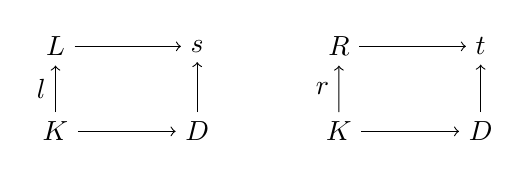
\begin{tikzpicture}[scale=0.9, baseline=(current bounding box.center)]
    \node (L) at (0,1.2) {$L$};
    \node (K) at (0,0) {$K$};
    \node (G) at (2,1.2) {$s$};
    \node (D) at (2,0) {$D$};
    \draw[->] (K) -- node[left] {$l$} (L);
    \draw[->] (K) -- (D);
    \draw[->] (L) -- (G);
    \draw[->] (D) -- (G);
    \node at (1,0.6) {$\ulcorner$};

    \node (R) at (4,1.2) {$R$};
    \node (K2) at (4,0) {$K$};
    \node (H) at (6,1.2) {$t$};
    \node (D2) at (6,0) {$D$};
    \draw[->] (K2) -- node[left] {$r$} (R);
    \draw[->] (K2) -- (D2);
    \draw[->] (R) -- (H);
    \draw[->] (D2) -- (H);
    \node at (5,0.6) {$\ulcorner$};
\end{tikzpicture}
\]
where the left square is a pushout complement and the right square is a pushout in $\mathcal{C}$. The RMG view treats $s$ and $t$ as objects in such a category, with DPO rewrites as morphisms.
\end{definition}

\begin{remark}[Rulial Space as a Free Category on a Rewrite Graph]
The underlying directed graph with vertex set $\mathcal{S}$ and edges $s \to t$ for each legal rewrite generates a free category $\mathcal{P}$ whose morphisms are rewrite paths. Rulial Distance $d(s,t)$ is then the length of the shortest non-identity morphism from $s$ to $t$, extended to $\infty$ when no such morphism exists. This endows the rewrite category with a canonical path-length pseudometric.
\end{remark}

\begin{conjecture}[Rulial Manifold Conjecture]
After suitable coarse-graining (e.g., quotienting by observational equivalence or collapsing high-frequency microscopic rewrites), large-scale regions of Rulial Space admit an effective description as a metric measure space with manifold-like properties. In this regime, discrete curvature as defined above should approximate a smooth curvature notion, yielding a bridge between computational geometry and classical differential geometry.
\end{conjecture}

\begin{remark}
If this conjecture holds even in restricted classes of RMGs, it opens the door to treating long-running computations as trajectories in an emergent geometric space, with optimization, scheduling, and verification all recast as geometric problems about geodesics, curvature, and volume.
\end{remark}

\section*{Forward References: Where These Structures Reappear}
\addcontentsline{toc}{section}{Forward References}

The formal machinery introduced in this appendix becomes essential in later parts of the book:

\begin{itemize}

\item \textbf{Part III: The Physics of C{\Large$\Omega$}MPUTER}  
      \begin{itemize}
          \item \textbf{Chapter \ref{chapter-9-curvature} (Curvature in MWMR)}\,:  
                The curvature definition $\kappa_{A,B}(s)$ becomes the core analytic tool for 
                describing “bottleneck regions” in multiway multi-rewrite (MWMR) dynamics.  
                The discrete energy landscape introduced here generalizes to higher-dimensional
                computational curvature.

          \item \textbf{Chapter 10 (Local NP Collapse)}\,:  
                The Rulial Distance $d(s,t)$ is used to formalize the notion of algorithmic 
                effort as a geometric quantity. NP-like behavior appears as regions of extremely 
                high curvature or narrow funnels in the future cones $F_k(s)$.

          \item \textbf{Chapter 11 (Rewrite Bundles and Superposition)}\,:  
                The future cone $F(s)$ and observer distance $D_k(\gamma_1,\gamma_2)$ define the 
                geometry over which rewrite bundles are superposed. Divergence of worldlines is 
                expressed using the pseudometric structure introduced here.

          \item \textbf{Chapter 12 (Interference and Collapse)}\,:  
                The categorical view of rewrites as morphisms in the free path category becomes 
                the substrate for defining interference, collapse, and observer-dependent dynamics.
      \end{itemize}

\item \textbf{Part V: The Compiler-Runtime Collapse}  
      \begin{itemize}
          \item The identity between storage and computation, and the metric interpretation 
                of rewrites, reappears when we show that compilation is equivalent to global 
                geodesic selection in Rulial Space.

          \item Curvature plays the role of “semantic resistance,” explaining optimization and 
                code motion as geometric transformations.
      \end{itemize}

\item \textbf{Appendices}  
      \begin{itemize}
          \item The categorical DPO formalism is expanded into a full algebraic semantics for 
                RMG rewriting, including adhesive-category properties, functorial semantics, 
                and conditions for confluence.
      \end{itemize}

\end{itemize}

\vspace{1em}

In summary, Rulial Space is not merely a metaphorical ``space of possibilities.'' It is a directed pseudometric space, enriched by an energy-like potential and a categorical DPO rewriting structure. Chronos traces geodesics in this space; Kairos reveals its local neighborhoods; Aios bounds the universe of legal states. Together, they endow computation with a genuine geometry.

\section{Transition: From Possibility to Path}
\label{transition-from-possibility-to-path}

We have established the vocabulary of the new world. We have seen the lens (Time Cube), the space (Aios), the actual path (Chronos), and the geometry (Rulial Distance). We can finally answer the question: \textbf{``What is execution, really?''}

Execution is not a mechanical ticking of a clock. Execution is \textbf{a worldline—a geodesic path through possibility space.}

Chapter 6 is where we quantify that path. It is where we talk about geodesics, deterministic observers, tick-level scheduling, and counterfactual timelines. It is where we explore how collapse works, how optimization is actually path-shortening, and how debugging is actually history traversal.

This is where computation becomes a \textbf{journey}, not a machine. And that is where we go next.

\section*{Symbol Glossary}
\addcontentsline{toc}{section}{Symbol Glossary}

\begin{center}
\begin{tabularx}{\linewidth}{@{}lX@{}}
\toprule
\textbf{Symbol} & \textbf{Meaning} \\
\midrule

$\mathcal{S}$ & The Rulial State Space: all states legal under the rule algebra $\mathcal{R}$. \\[2pt]

$\mathcal{R}$ & The DPO rule algebra governing legal rewrites in the RMG universe. \\[2pt]

$s \to t$ & A legal one-step rewrite from $s$ to $t$ (Chronos step). \\[2pt]

$N(s)$ & The \emph{Kairos slice} or local neighborhood: all states reachable in one step from $s$. \\[2pt]

$d(s,t)$ & \textbf{Rulial Distance}: minimal number of rewrites required to transform $s$ into $t$; \\ 
         & equals $\infty$ if no such sequence exists. \\[2pt]

$F_k(s)$ & The $k$-step future cone: all states reachable from $s$ in exactly $k$ rewrites. \\[2pt]

$F(s)$ & The full future cone: $\bigcup_{k \ge 0} F_k(s)$, all reachable futures under $\mathcal{R}$. \\[2pt]

$\gamma$ & A worldline (execution): $s_0 \to s_1 \to s_2 \to \dots$ \\[2pt]

$D_k(\gamma_1, \gamma_2)$ & Observer distance: divergence of two worldlines over $k$ steps. \\[2pt]

$E(s)$ & Effort potential: minimal distance to a locally stable state. \\[2pt]

Stable Basin & A region of state space where rewrites naturally converge toward a \\
            & specific attractor or normal form (low curvature). \\[2pt]

$\kappa_{A,B}(s)$ & Rulial curvature at $s$ between basins $A$ and $B$; the activation barrier height. \\[2pt]

$\Gamma(s \to B)$ & All rewrite paths from $s$ into the basin of $B$. \\[2pt]

$L \xleftarrow{l} K \xrightarrow{r} R$ & A DPO rule: left-hand side $L$, interface $K$, right-hand side $R$. \\[2pt]

\bottomrule
\end{tabularx}
\end{center}

\vspace{1em}
